% Focused tkz-euclide result-ordering regression derived from the Thales fixture.
% `common=C` must leave C in the second tkzGetPoints result.
\documentclass[border=2pt]{standalone}
\usepackage{tikz}
\usepackage{tkz-euclide}
\begin{document}
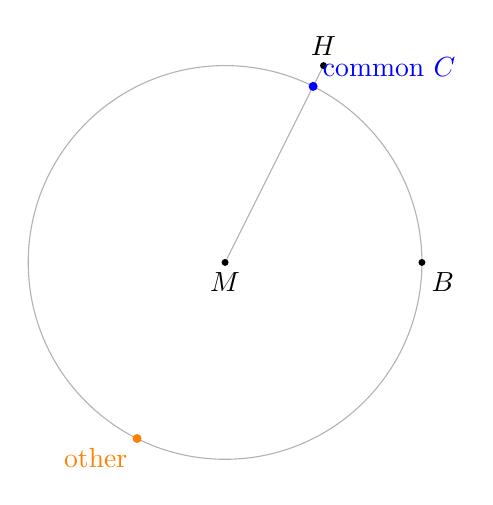
\begin{tikzpicture}[scale=1.25]
  \tkzDefPoint(2,0){M}
  \tkzDefPoint(4,0){B}
  \tkzDefPoint(3,2){H}
  \tkzInterLC(M,H)(M,B) \tkzGetPoints{E}{C}
  \tkzInterLC[common=C](C,H)(M,B) \tkzGetPoints{Other}{Common}

  \draw[color=gray!60] (M) circle (2cm);
  \draw[gray!60] (M) -- (H);
  \fill (M) circle (1pt) (B) circle (1pt) (H) circle (1pt);
  \fill[blue] (Common) circle (1.3pt);
  \fill[orange] (Other) circle (1.3pt);
  \node[below] at (M) {$M$};
  \node[below right] at (B) {$B$};
  \node[above] at (H) {$H$};
  \node[above right,blue] at (Common) {common $C$};
  \node[below left,orange] at (Other) {other};
\end{tikzpicture}
\end{document}
